\section{Image Processing Applications}
\label{sec:imageProcessing}
Many image processing applications are inherently parallel as they often independently process the pixels of an image.
Common examples range from simple thresholding over noise reduction applications to techniques used in edge detection and pattern recognition~\cite{Umbaugh1997}.
In this section we will study three application examples from image processing and how they can be implemented using \SkelCL.

We start by looking at the Gaussian blur application which reduces noise in images and is often used as a preprocessing step in more complex algorithms.
We will then discuss two algorithms used for edge detection in images:
the Sobel edge detection application and the more complex Canny edge detection algorithm.

These three applications can be expressed using the \stencil skeleton introduced in \autoref{section:skelcl-programming-model:specialSkeletons}, but they have different characteristics.
The Gaussian blur applies a single stencil computation, possibly iterated multiple times, for reducing the noise in images.
The Sobel edge detection applies a stencil computation once to detect edges in images.
The more advanced Canny edge detection algorithm consists of a sequence of stencil operations which are applied to obtain the final result.
For each of the three applications, we compare the performance using our two implementations of the \stencil skeleton:
\code{MapOverlap} and \code{Stencil} with native OpenCL implementations using an input image of size $4096 \times 3072$.










\subsection{Gaussian Blur}
\label{sec:gauss}
The Gaussian blur is a standard algorithm used in image processing~\cite{Umbaugh1997}.
One common application is reduction of image noise as shown in \autoref{fig:lena:noise}.
%
\begin{figure}[tb]
  \centering
  \begin{subfigure}[t]{.45\textwidth}
    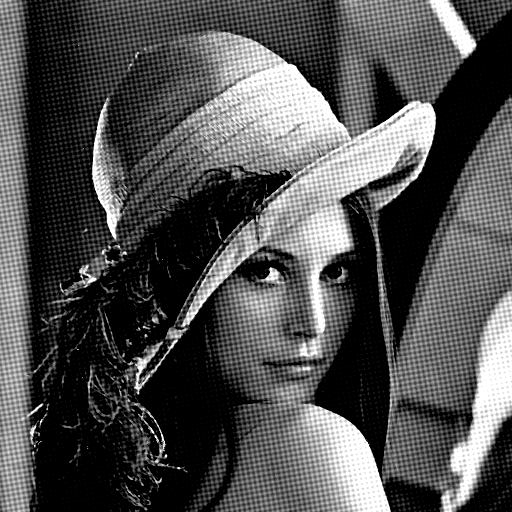
\includegraphics[width=\textwidth]{lenaNoise}
    \caption{The Lena image with noise.}
    \label{fig:lena:noise:yes}
  \end{subfigure}
  \hfill
  \begin{subfigure}[t]{.45\textwidth}
    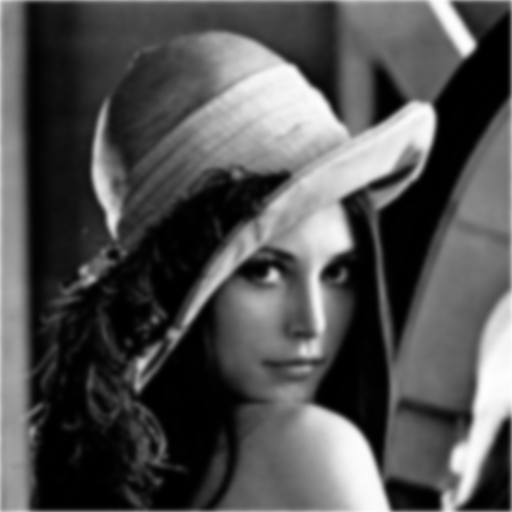
\includegraphics[width=\textwidth]{lenaNoNoise}
    \caption{The Lena image after applying the Gaussian blur.}
    \label{fig:lena:noise:no}
  \end{subfigure}
  \caption{Effect of applying the Gaussian blur to an noised image.}
  \label{fig:lena:noise}
\end{figure}
%
The image~\cite{} on the left has some noise as it is typically produced by halftone printing used to print newspapers.
The Gaussian blur has been applied to reduce the noise and produce the image on the right.

The Gaussian blur computes the color of every pixel using a weighted average of the neighboring pixel color values.
Using \SkelCL this application can easily be expressed using the \stencil skeleton.

\subsubsection*{\SkelCL Implementation}
\autoref{eq:gauss} shows the implementation in \SkelCL using the \stencil skeleton.
\begin{align}
  gauss&\ M = stencil\ f\ 1\ \overline{0}\ M \qquad\text{where:}\nonumber\\
  &
  \begin{array}{ll}%
  f\ &\left[\begin{array}{lll}%
      \hspace{-.5em} M_{i-1,j-1}& \hspace{-.5em} M_{i-1,j} & \hspace{-.5em}M_{i-1,j+1}\vspace{-.25em}\\%
      \hspace{-.5em} M_{i,j-1}& \hspace{-.5em} M_{i,j} & \hspace{-.5em}M_{i,j+1}\vspace{-.25em}\\%
      \hspace{-.5em} M_{i+1,j-1}& \hspace{-.5em} M_{i+1,j} & \hspace{-.5em}M_{i+1,j+1}
    \end{array}\right]  = \\[2em]
          &\qquad \displaystyle\frac{\displaystyle\sum_{k=-1}^{1} \sum_{l=-1}^{1} (G\ k\ l)\cdot M_{i+k, j+k}}{9},
  \end{array} \label{eq:gauss}\\[1em]
  &G\ x\ y = \frac{1}{2\pi \sigma^{2}} e^{-\frac{x^2 + y^2}{2\sigma^2}} \nonumber\\
  \text{and } \overline{0} \text{ is th}&\text{e constant function always returning zero.}\nonumber
\end{align}
$G$ is the two-dimensional Gaussian function used in the customizing function $f$ to weight the neighboring values $M_{i,j}$.
The values obtained by applying $G$ can be precomputed, as $G$ is only evaluated with values in the interval $[-1, 1]$ for $x$ and $y$.


\autoref{lst:skelcl:gauss} shows the \SkelCL-based implementation of the Gaussian blur using the \code{MapOverlap} implementation of the \stencil skeleton.
Here the immediate neighboring pixels are accessed (lines~\ref{lst:skelcl:gauss:start}--\ref{lst:skelcl:gauss:end}) and used to compute a weighted value for each pixel.
The function computing the weighted sum is omitted here.
It is also possible to extend the \emph{range} of the Gaussian blur and include more neighboring pixel values in the computation.

\begin{lstlisting}[%                                                             
caption={Implementation of the Gaussian blur in \SkelCL using the \code{MapOverlap} implementation of the \stencil skeleton.},%
numbers=left,%
float=tb,
label={lst:skelcl:gauss}]
Matrix<char> gaussianBlur(const Matrix<char>& image) {
  auto gauss = mapOverlap(
    [](Neighborhood<char>& in) {
      char ul = in[{-1, -1}];$\label{lst:skelcl:gauss:start}$
      ...
      char lr = in[{+1, +1}];$\label{lst:skelcl:gauss:end}$
      return computeGaussianBlur(ul, ..., lr); },
    1, BorderHandling::NEUTRAL(0));
  return gauss(image); }
\end{lstlisting}

\subsubsection*{Programming effort}

\begin{figure}[tbp]
	\centering
	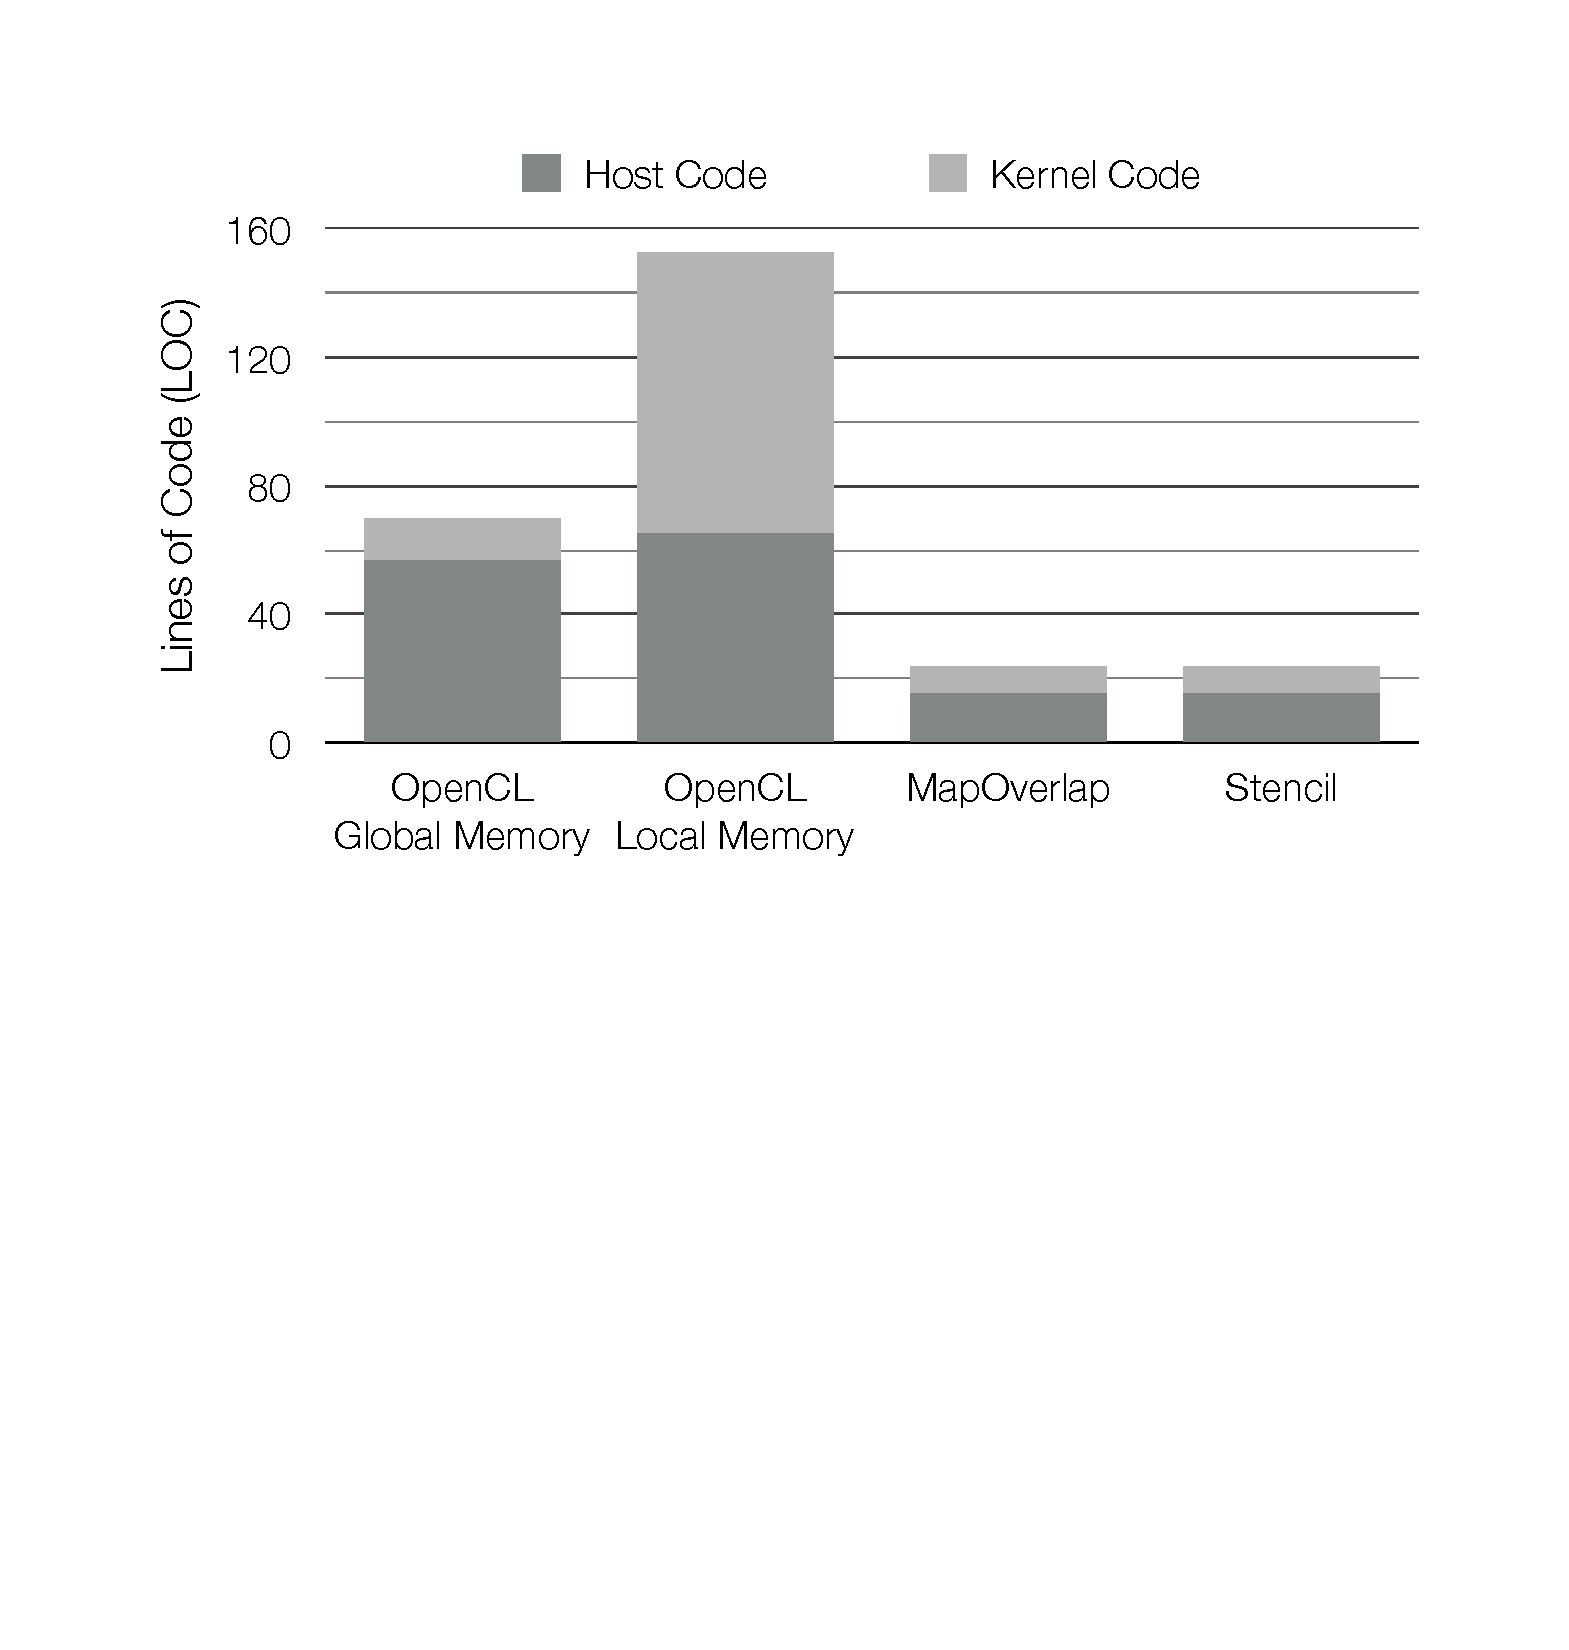
\includegraphics[width=\columnwidth]{HiStencils/LOC.pdf}
	\caption[Lines of code of the Gaussian blur using different implementations.]%
          {Lines of code of the Gaussian blur using a na{\"i}ve OpenCL implementation with global memory, an optimized OpenCL version using local memory, and \SkelCL's \code{MapOverlap} and \code{Stencil} implementations of the \stencil skeleton.}
	\label{fig:gaussLOCs}
\end{figure} 

\autoref{fig:gaussLOCs} shows the program sizes (in lines of code) for the four implementations of the Gaussian blur. 
The application developer needs $57$ lines of OpenCL host code and 13 LOCs for performing a Gaussian blur with global memory. 
When using local memory, some more arguments are passed to the kernel, thus, increasing the host-LOCs to $65$, while the LOCs for the kernel function, which copies all necessary elements for a work-group's calculation into local memory, requires $88$ LOCs including explicit out-of-bounds handling and complex index calculations.
The \code{MapOverlap} and \code{Stencil} versions are similar and both require only $15$ LOCs host code and $9$ LOCs kernel code to perform a Gaussian blur. 
The support for multi-\GPU systems is implicitly provided when using \SkelCL's skeletons, such that the kernel remains the same as for one-\GPU systems.
This is an important advantage of \SkelCL over the \OpenCL implementations of the Gaussian blur which are single-\GPU only, and they require additional LOCs when fitting to multi-\GPU environments.

The implementations using \code{MapOverlap} and \code{Stencil} are only $5-10\%$ slower than an optimized OpenCL implementation of the Gaussian blur while being much shorter than the OpenCL version.

\subsubsection*{Performance experiments}

\begin{figure}[tbp]
	\centering
	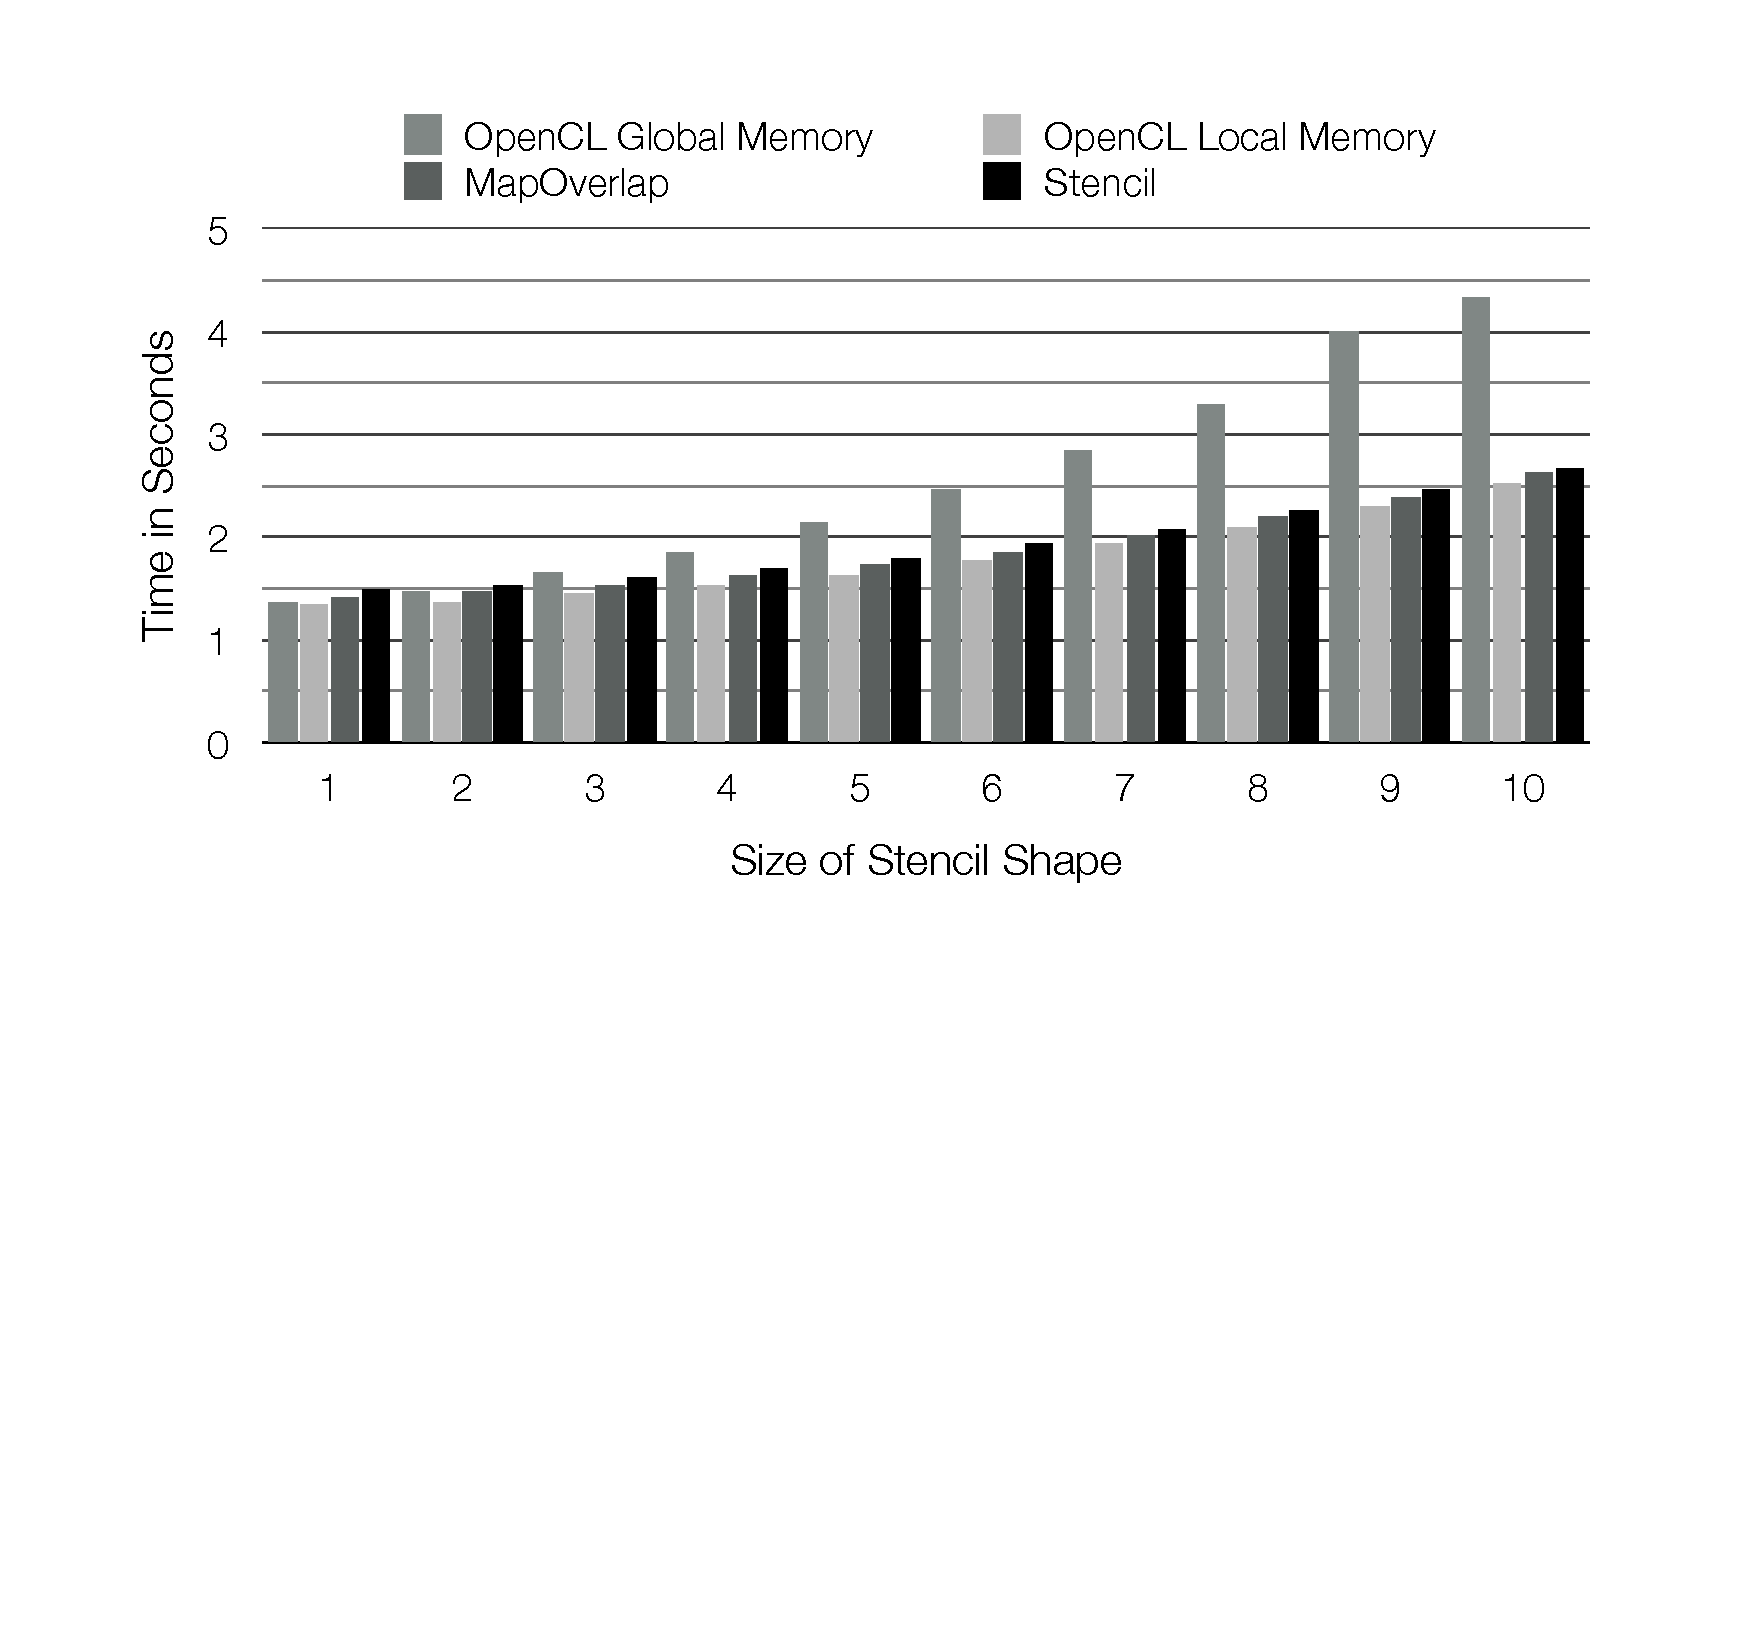
\includegraphics[width=\columnwidth]{HiStencils/GaussOpenCL.pdf}
	\caption[Runtime of the Gaussian blur using different implementations.]%
          {Runtime of the Gaussian blur using a na{\"i}ve OpenCL implementation with global memory, an OpenCL version using local memory and SkelCL's MapOverlap and Stencil skeletons.}
	\label{fig:gaussAbs}
\end{figure} 

\autoref{fig:gaussAbs} shows the measured total runtime of the Gaussian blur using:
\begin{itemize}
  \item[1)] a na{\"i}ve OpenCL implementation using global memory,
  \item[2)] an optimized OpenCL version using local memory,
  \item[3)] \code{MapOverlap}-based implementation, and
  \item[4)] the \code{Stencil}-based implementation, correspondingly.
\end{itemize}
We observe that for larger stencil shape sizes, the \code{MapOverlap} and \code{Stencil}-based versions outperform the na{\"i}ve OpenCL implementation by $65\%$ and $62\%$, respectively.
The optimized OpenCL version, which copies all necessary elements into local memory prior to calculation, is $5\%$ faster than \code{MapOverlap} and $10\%$ faster than \code{Stencil} for small stencil shapes.
When increasing the stencil shape size, this disadvantage is reduced to $3\%$ for \code{MapOverlap} and $5\%$ for \code{Stencil} with stencil shape's extent of $10$ in each direction.

The \code{Stencil} implementation is slower for small stencil shapes than the \code{MapOverlap} implementation, up to $32\%$ slower for an stencil shape size of $1$.
This is due to the increased branching required in the \code{Stencil} implementation, as discussed in more detail in \autoref{sec:skelcl:stencil}.
However, this disadvantage is reduced to $4.2\%$ for the stencil shape size of $5$ and becomes negligible for bigger stencil shape sizes.
% Due to the increased branching in Stencil's kernel function, one might expect a worse runtime for the Stencil skeleton. 
As the ratio of copying into local memory decreases in comparison to the number of calculations when enlarging the stencil shape's extents, the kernel function's runtime in the \code{Stencil} implementation  converges to the \code{MapOverlap} implementation's time.
The \code{Stencil} implementation's disadvantage is also due to its ability to manage multiple stencil shapes and explicitly support the use of iterations.
While both features are not used in this application example, they incur some overhead for the implementation as compared to the \code{MapOverlap} implementation for simple stencil computations.


\autoref{fig:GaussMult} shows the speedup achieved on the Gaussian blur using the \code{Stencil} implementation on up to four devices.
The higher the computational complexity for increasing size of stencil shape, the better the overhead is hidden, leading to a maximum speedup of $1.90$ for two devices, $2.66$ for three devices, and $3.34$ for four devices.
\begin{figure}
	\centering
	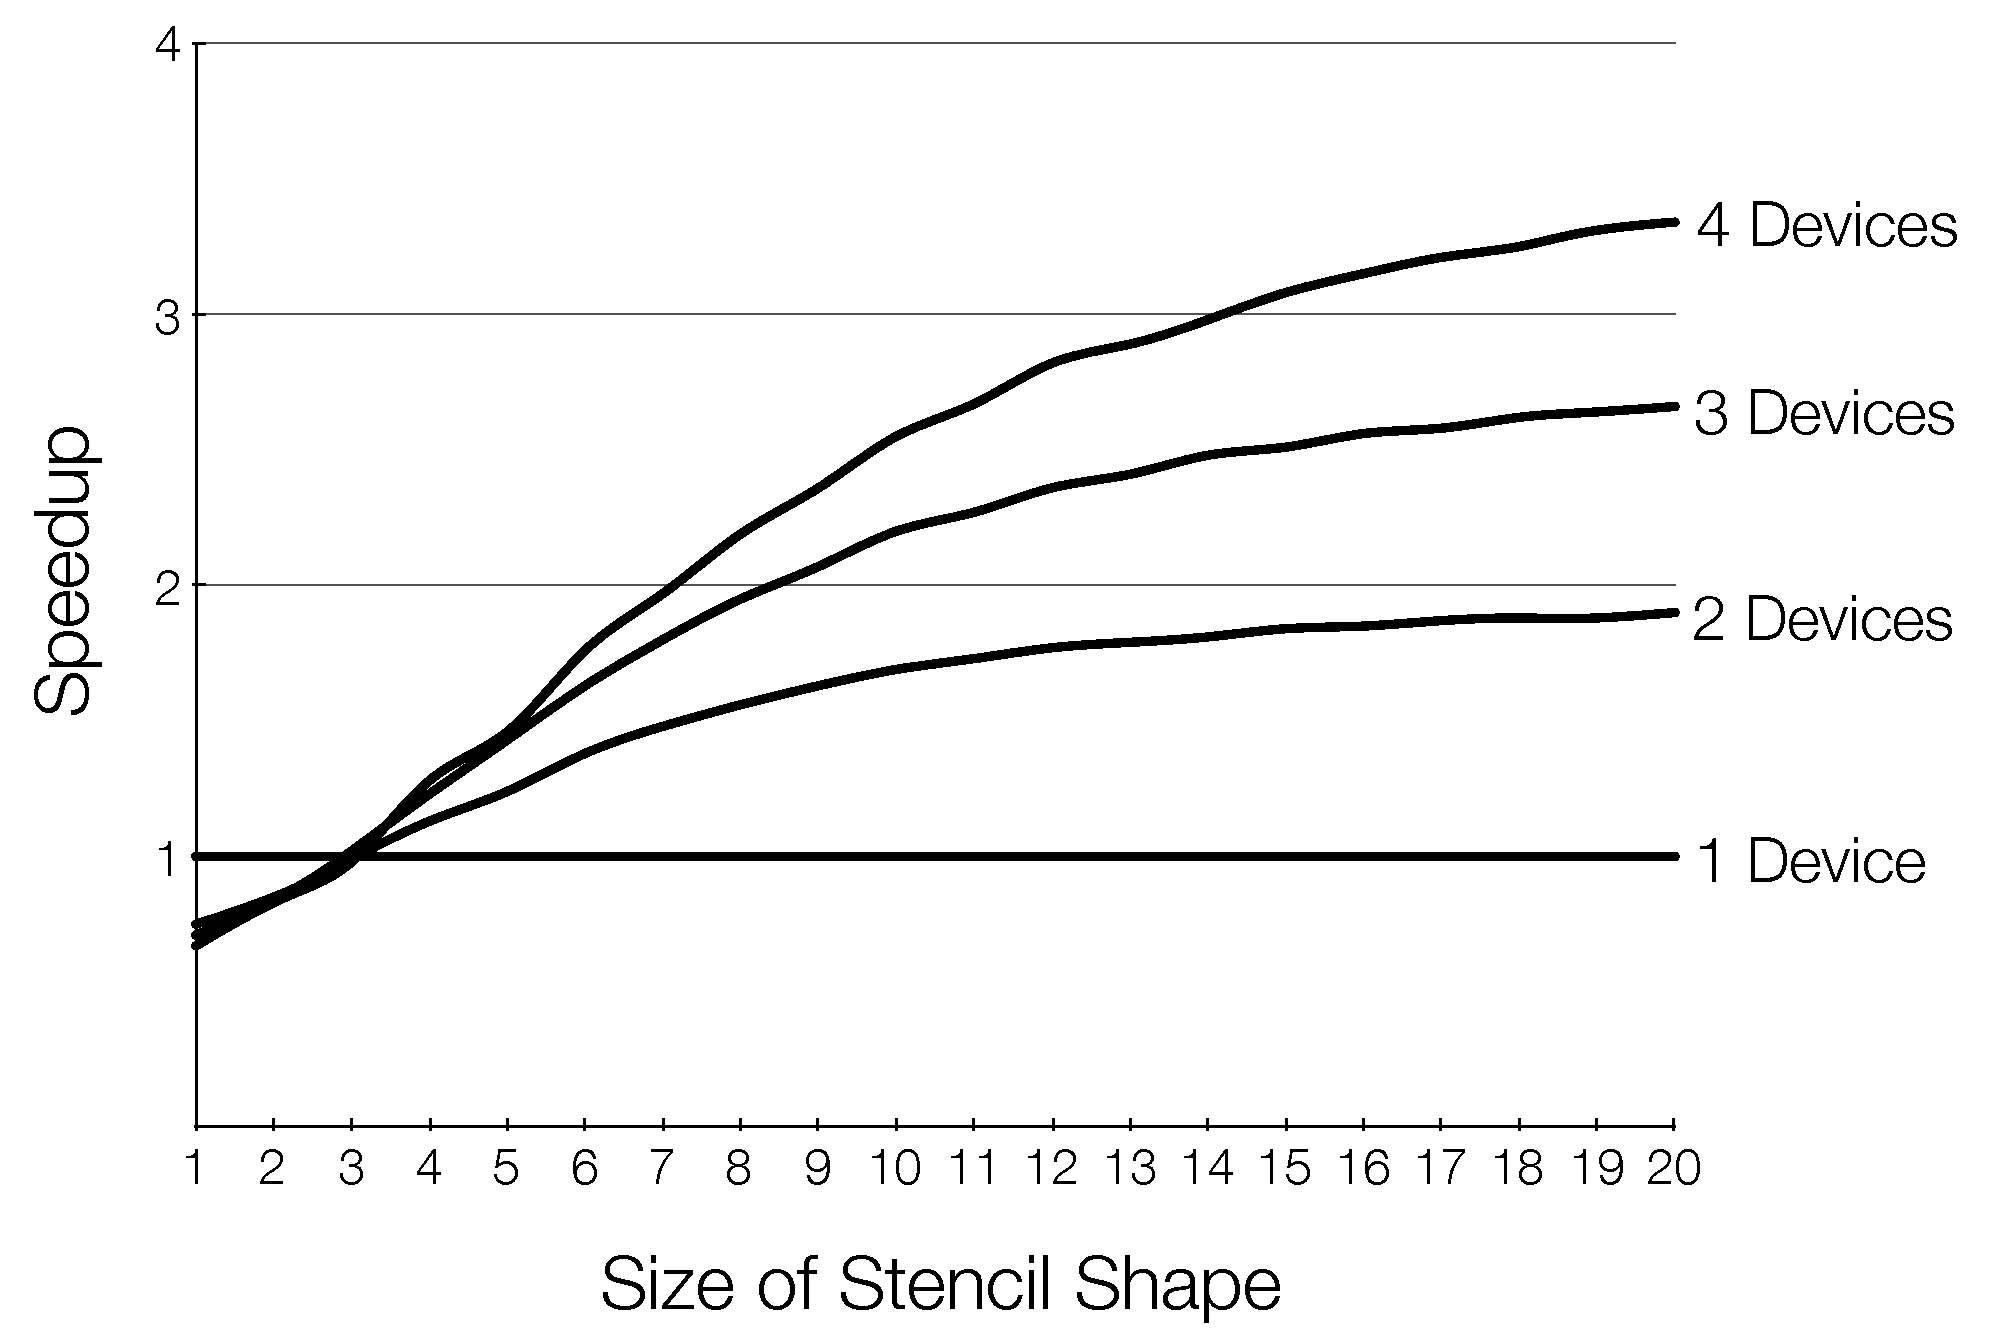
\includegraphics[width=.85\columnwidth]{HiStencils/SpeedupGauss.pdf}
	\caption{Speedup of the Gaussian blur application on up to four \GPUs.}
	\label{fig:GaussMult}
\end{figure} 










\subsection{Sobel Edge Detection}
\label{sec:sobel}
The Sobel edge detection produces an output image in which the detected edges in the input image are marked in white and plain areas are shown in black.
The effect is shown in \autoref{fig:sobel:lena}, where the original image is shown on the left and the output of Sobel edge detection applied to it on the right.

\begin{figure}[tb]
  \centering
  \begin{subfigure}[t]{.45\textwidth}
    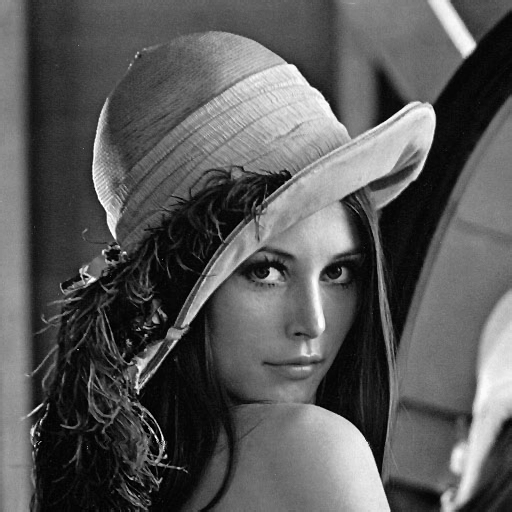
\includegraphics[width=\textwidth]{Paraphrase/lena.png}
    \caption{Original image.}
    \label{fig:lena:orig}
  \end{subfigure}
  \hfill
  \begin{subfigure}[t]{.45\textwidth}
    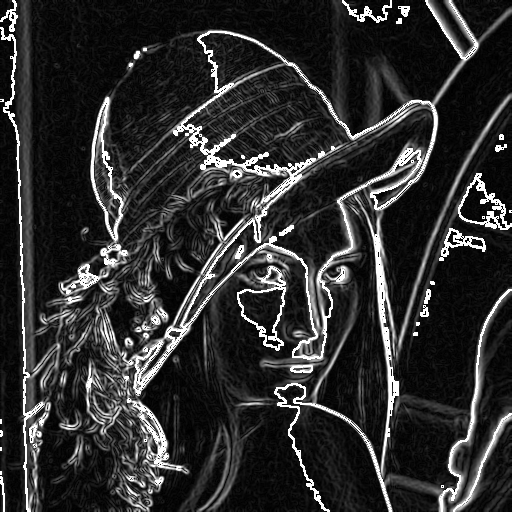
\includegraphics[width=\textwidth]{Paraphrase/sobel_filtered-lena.png}
    \caption{Image after Sobel edge detection.}
    \label{fig:lena:sobel}
  \end{subfigure}
  \caption[The Lena image before and after applying Sobel edge detection.]%
          {The Lena image~\cite{Lena} often used as an example in image processing before (left) and after (right) applying Sobel edge detection.}
  \label{fig:sobel:lena}
\end{figure}

\begin{lstlisting}[%
caption={Sequential implementation of the Sobel edge detection.},%
float=tb,
label={lst:sobel:seq}]
for (i = 0; i < width; ++i)
  for (j = 0; j < height; ++j)
    h = -1*img[i-1][j-1] +1*img[i+1][j-1]
        -2*img[i-1][j  ] +2*img[i+1][j  ]
        -1*img[i-1][j+1] +1*img[i+1][j+1];
    v = ...;
    out_img[i][j] = sqrt(h*h + v*v);
\end{lstlisting}
\bigskip

\autoref{lst:sobel:seq} shows the sequential algorithm of the Sobel edge detection in pseudo-code, with omitted boundary checks for brevity.
In this version, for computing an output value \code{out\_img[i][j]} the input value \code{img[i][j]} and the direct neighboring elements are needed.
Therefore, the \stencil skeleton is a perfect fit for implementing the Sobel edge detection.

\subsubsection*{\SkelCL Implementation}
\autoref{eq:sobel} shows the implementation of the Sobel edge detection in the \SkelCL programming model.
\begin{align}
  \label{eq:sobel}
  sobel\ M& = stencil\ f\ 1\ \overline{0}\ M \qquad\text{where:}\\
  f\ &\left[\begin{array}{lll}%
      \hspace{-.5em} M_{i-1,j-1}& \hspace{-.5em} M_{i-1,j} & \hspace{-.5em}M_{i-1,j+1}\vspace{-.25em}\\%
      \hspace{-.5em} M_{i,j-1}& \hspace{-.5em} M_{i,j} & \hspace{-.5em}M_{i,j+1}\vspace{-.25em}\\%
      \hspace{-.5em} M_{i+1,j-1}& \hspace{-.5em} M_{i+1,j} & \hspace{-.5em}M_{i+1,j+1}
    \end{array}\right] = \displaystyle\sqrt{ h^2 + v^2 }\nonumber\\
  h & = \sum_{k=0}^2 \sum_{l=0}^2 Gx_{k, l}\cdot M_{i+k-1,j+k-1}\nonumber\\
  v & = \sum_{k=0}^2 \sum_{l=0}^2 Gy_{k, l}\cdot M_{i+k-1,j+k-1}\nonumber\\
  Gx& = \left[\begin{array}{ccc}%
      -1&0&+1\\
      -2&0&+2\\
      -1&0&+1
    \end{array}\right]
  Gy = \left[\begin{array}{ccc}%
      -1&-2&-1\\
      0&0&0\\
      +1&+2&+1
    \end{array}\right] \nonumber\\
  \text{and } \overline{0} \text{ is th}&\text{e constant function always returning 0.}\nonumber
\end{align}
The formula resembles the sequential implementation shown in \autoref{lst:sobel:seq} where the final result is computed as the square root of the sum of two squared terms $h$ and $v$.
These are computed as weighted sums of the neighboring values $M_{i,j}$.
The weights are given by the two matrices $Gx$ and $Gy$.

\autoref{lst:sobel:skelcl} shows the \SkelCL implementation using the \code{MapOverlap} implementation of the \stencil skeleton.
%
\begin{lstlisting}[%
caption={\SkelCL implementation of the Sobel edge detection.},%
numbers=left,
float=tb,
label={lst:sobel:skelcl}]
Matrix<char> sobelEdge(const Matrix<char>& image) {
  auto sobel = mapOverlap(
    [](Neighborhood<char>& in) {
      short h = -1*in[{-1,-1}] +1*in[{+1,-1}]
                -2*in[{-1, 0}] +2*in[{+1, 0}]
                -1*in[{-1,+1}] +1*in[{+1,+1}];
      short v = ...;
      return sqrt(h*h + v*v); },
    1, BorderHandling::NEUTRAL(0));
  return soble(img); }
\end{lstlisting}
%
The implementation is straightforward and very similar to the formula in \autoref{eq:sobel} and the sequential version in \autoref{lst:sobel:seq}.

\subsubsection*{Programming effort}

\begin{lstlisting}[%
caption={Additional boundary checks and index calculations for Sobel algorithm, necessary in the standard OpenCL implementation.},%
float=tb,
numbers=left,
label={lst:sobel:opencl}]
kernel void sobel_kernel( global const uchar* img,
                          global       uchar* out_img) {
 uint i = get_global_id(0);   uint j = get_global_id(1);
 uint w = get_global_size(0); uint h = get_global_size(1);
 // perform boundary checks
 if(i >= 1 && i < (w-1) && j >= 1 && j < (h-1)) {
  char ul = img[((j-1)*w)+(i-1)];
  char um = img[((j-1)*w)+(i+0)];
  char ur = img[((j-1)*w)+(i+1)];
  // ... 5 more
  char lr = img[((j+1)*w)+(i+1)];

  out_img[j * w + i] = computeSobel(ul, um, ur, ..., lr); }}
\end{lstlisting}

\autoref{lst:sobel:opencl} shows a part of the rather simple \OpenCL implementation for Sobel edge detection provided by AMD as an example for their software development kit~\cite{AMDSDK}.
The actual computation is performed inside the \texttt{computeSobel} function, which is omitted in the listing, since it is quite similar to the sequential version in \autoref{lst:sobel:seq}.
The listing shows that extra low-level code is necessary to deal with technical details, like boundary checks and index calculations, which are arguably quite complex and error-prone.

We also compare against a more optimized \OpenCL implementation by Nvidia which makes use of the fast local \GPU memory.

The \SkelCL implementation is significantly shorter than the two \OpenCL-based implementations.
The \SkelCL program only comprises few lines of code as shown in \autoref{lst:sobel:skelcl}.
The AMD implementation requires 37 lines of code for its kernel implementation and the more optimized Nvidia implementation requires even 208 lines of code.
Both versions require additional lines of code for the host program which manages the execution of the \OpenCL kernel.
No index calculations or boundary checks are necessary in the \SkelCL version whereas they are crucial for a correct implementation in \OpenCL.

\subsubsection*{Performance experiments}

\begin{figure}[tbp]
  \vspace{.5em}
  \centering
  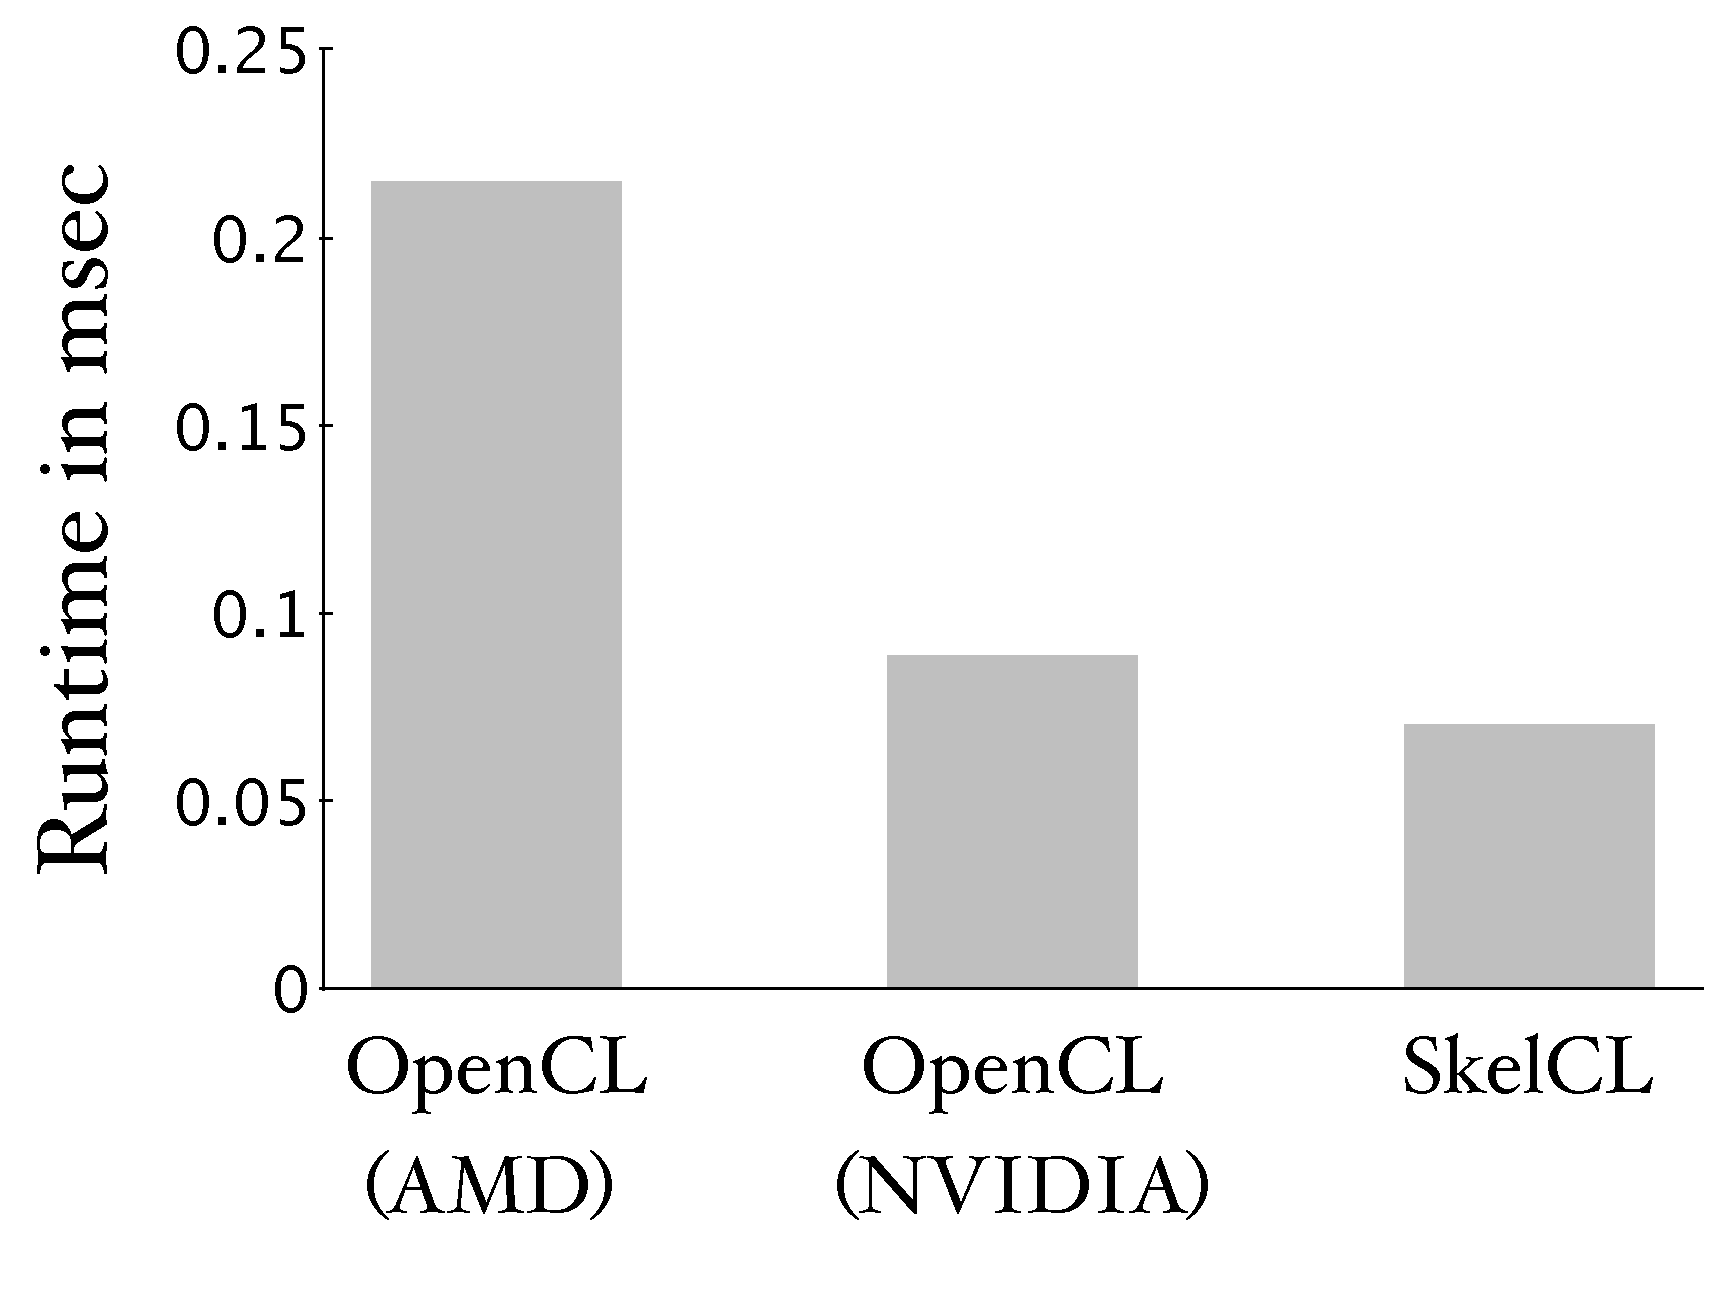
\includegraphics[height=4.5cm]{PaCT/lena.pdf}
  \caption{Performance results for Sobel edge detection}
  \label{fig:sobel:measurements}
\end{figure}
\autoref{fig:sobel:measurements} shows the measured runtime of two \OpenCL versions (from the AMD and Nvidia SDKs) vs. the \SkelCL version with the \stencil skeleton presented in \autoref{lst:sobel:skelcl}.
Here only the kernel runtimes are shown, as the data transfer times are equal for all versions.
We used the popular Lena image~\cite{Lena} with a size of $512\times 512$ pixel as an input.
The AMD version is clearly slower than the two other implementations, because it does not use the fast local memory which the Nvidia implementation and the \code{MapOverlap} implementation of the \stencil skeleton of \SkelCL do.
\SkelCL completely hides the memory management details inside its implementation from the application developer.
The Nvidia and \SkelCL implementations perform similarly fast.
In this particular example, \SkelCL even slightly outperforms the implementation by Nvidia.










\subsection{Canny Edge Detection}
The Canny edge detection algorithm is a more complex algorithm to detect edges in images than the Sobel edge detection presented in the previous section.
For the sake of simplicity we consider a slightly simplified version, which applies the following stencil operations in a sequence:
1), a noise reduction operation is applied, \eg, a Gaussian blur;
2), an edge detection operator like the Sobel edge detection is applied;
3), the so-called non-maximum suppression is performed, where all pixels in the image are colored black except pixels being a local maximum;
4), a threshold operation is applied to produce the final result.
A more complex version of the algorithm performs the edge tracking by hysteresis, as an additional step.
This results in detecting some weaker edges, but even without this additional step the algorithm usually achieves good results.


\subsubsection*{\SkelCL Implementation}
In \SkelCL, each single step of the Canny algorithm can be expressed using the \stencil skeleton.
The last step, the threshold operation, does not need access to neighboring elements, as the user threshold function only checks the value of the current pixel.
Therefore, this step can be expressed using \SkelCL's simpler \map skeleton.
In the \SkelCL library the \code{Stencil} skeleton's implementation automatically uses the simpler \map skeleton's implementation when the user specifies a stencil shape which extents are $0$ in all directions.

\begin{lstlisting}[%
  caption={Structure of the Canny algorithm expressed as a sequence of skeletons.},%
  float=tbp,%
  label={lst:skelcl:canny}]
Matrix<char> sobelEdge(const Matrix<char>& image) {
  auto gauss     = stencil(...);$\label{lst:skelcl:canny:step1}$
  auto sobel     = stencil(...);
  auto nms       = stencil(...);
  auto threshold = stencil(...);$\label{lst:skelcl:canny:stepN}$
  StencilSequence<Pixel(Pixel)>
      canny(gauss, sobel, nms, threshold);$\label{lst:skelcl:canny:combine}$
  return canny(image); }$\label{lst:skelcl:canny:call}$
\end{lstlisting}

To implement the Canny algorithm in \SkelCL, the single steps can be combined as shown in \autoref{lst:skelcl:canny}.
The individual steps are defined in lines~\ref{lst:skelcl:canny:step1}--\ref{lst:skelcl:canny:stepN} and then combined to a sequence of stencils in line~\ref{lst:skelcl:canny:combine}.
During execution (line~\ref{lst:skelcl:canny:call}), the stencil operations are performed in the order which is specified when creating the \emph{StencilSequence} object.

%\subsubsection*{Programming effort}

\subsubsection*{Performance experiments}

\begin{figure}[tbp]
	\centering
	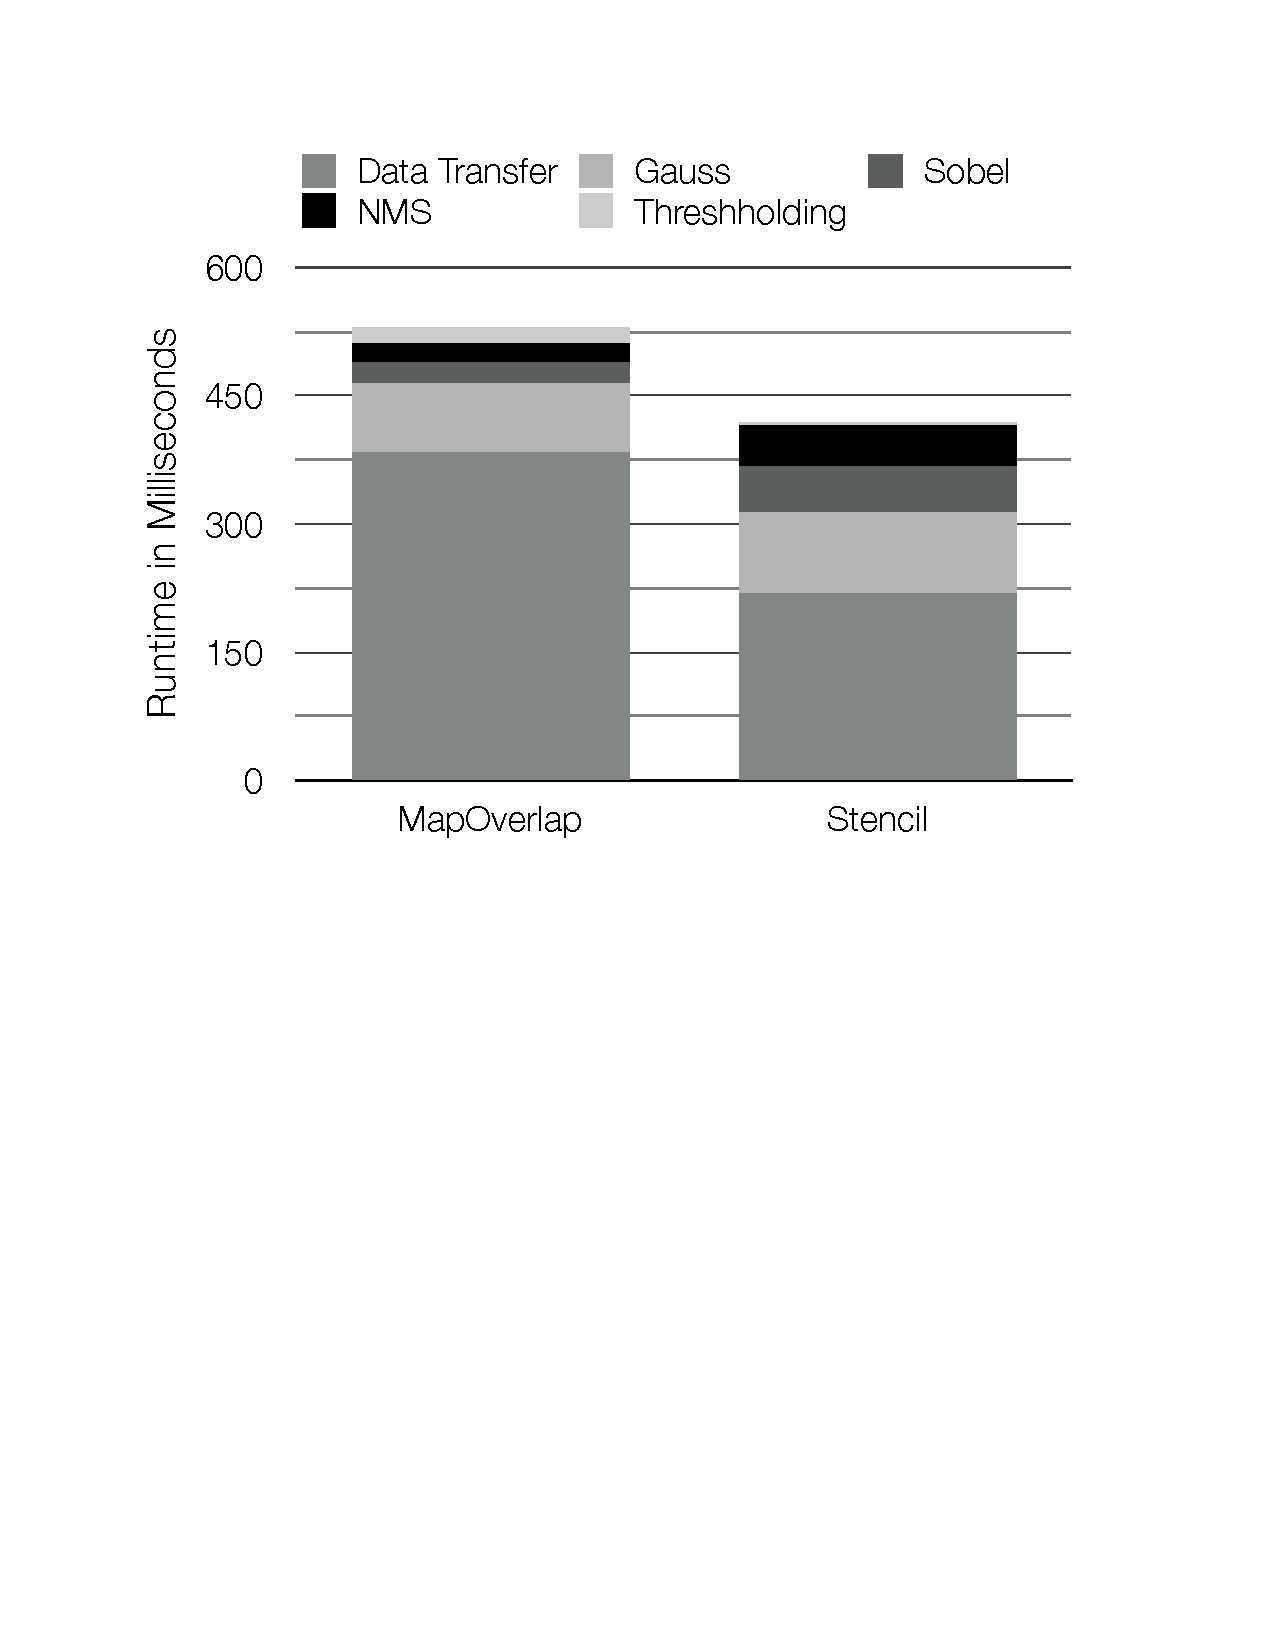
\includegraphics[width=.9\columnwidth]{HiStencils/Canny.pdf}
	\caption[Runtime of the Canny edge detection algorithm.]%
          {Runtime of the Canny edge detection algorithm comparing the \code{MapOverlap} and \code{Stencil} skeleton implementations.}
	\label{fig:canny}
\end{figure} 

\autoref{fig:canny} shows the measured runtime of the Canny algorithm using the two presented implementations.
As the \code{MapOverlap} implementation appends padding elements to the matrix, the matrix has to be downloaded, resized and uploaded again to the \GPU between every two steps of the sequence.
This additional work leads to an increased time for data transfers. 
The Gaussian blur with a stencil shape extent of $2$, as well as the Sobel edge detection and the non-maximum suppression with a stencil shape of $1$, are $2.1$ to $2.2$ times faster when using \code{MapOverlap}. 
However, the threshold operation, which is expressed as the \map skeleton in the Stencil sequence, is $6.8$ times faster than \code{MapOverlap}'s threshold operation.
Overall, we observe that when performing sequences of stencil operations, the \code{Stencil} implementation reduces the number of copy operations and, therefore, leads to a better overall performance.
When performing the Canny algorithm, the \code{Stencil} implementation outperforms the \code{MapOverlap} implementation by $21\%$.

